\begin{comment}
  http://www.visitusers.org/index.php?title=Running_client-server
\end{comment}

%% \begin{frame}{Distributed and remote visualization with VisIt}{}
%%   \begin{itemize}\setlength{\itemsep}{2mm}
%%   \item Working with fully remote VisIt
%%     \begin{itemize}\setlength{\itemsep}{0mm}
%%     \item ssh X-forwarding (X11 through ssh)
%%     \item remote VNC desktop
%%     \end{itemize}
%%   \item Client-server (remote VisIt server, local VisIt client)
%%   \item Parallel rendering
%%   \end{itemize}
%% \end{frame}

\begin{frame}{Visualizing remote data}
  So far we covered working with standalone VisIt on your desktop. If your dataset is on
  cluster.consortium.ca, you have many options to visualize it:\medskip
  \begin{enumerate}\setlength{\itemsep}{2mm}
  \item download data to your desktop and visualize it locally\\
    {\color{red} limited by dataset size and your desktop's CPU+GPU/memory}
  \item run VisIt remotely on a larger machine via X11 forwarding\\
    {\color{blue} your desktop $^{\underrightarrow{\rm ssh~-X}}$ larger machine running VisIt}
  \item run VisIt remotely on a larger machine {\bf via VNC}\\
    {\color{blue} your desktop $^{\underrightarrow{\rm VNC}}$ larger machine running VisIt}
    \begin{itemize}\setlength{\itemsep}{0mm}
    \item any node; preferably a GPU compute node
    \end{itemize}
  \item run VisIt in {\bf client-server mode}\\
    {\color{blue} VisIt viewer on your desktop $\rightleftharpoons$ VisIt on larger machine}
  \item run VisIt via a GUI-less batch script (interactively or scheduled)
  \end{enumerate}
  %% \medskip
  %% {\footnotesize
  %%   For remote options (2) - (5) the setup details vary across the consortia
  %%   \begin{itemize}\setlength{\itemsep}{0mm}
  %%   \item[-] render server can run with or without GPU rendering
  %%   \item[-] data/render servers can run on a single core, or across many cores/nodes with MPI
  %%   \item[-] for interactive GUI work on clusters it's best to schedule interactive jobs, as opposed to
  %%     running on the login nodes
  %%   \end{itemize}}
\end{frame}

\begin{frame}{X11 forwarding}
  \begin{itemize}\setlength{\itemsep}{3mm}
  \item Need a local X11 server (comes by default on Linux and Mac laptops) to which a remote application
    sends its window
  \item \hi{ssh -X} lets you forward X11 graphics and mouse/keyboard interactions through ssh (encrypted!)
  \item Can forward through several consecutive connections, e.g.\\ laptop $^{\underrightarrow{\rm
      ssh~-X}}$ login node $^{\underrightarrow{\rm ssh~-X}}$ interactive development node
    \pause
  \item X11 forwarding is very chatty (lots of roundtrips!) and can be very slow on a high-latency
    network ... in general we don't recommend it
  \end{itemize}
\end{frame}

\begin{frame}{VNC (Virtual Network Computing)}
  \begin{itemize}\setlength{\itemsep}{3mm}
  \item Remote graphical desktop system
  \item Has gone to tremendous effort to optimize communication via data compression and caching
  \item Best to use VNC via an SSH tunnel and with a non-empty VNC password for higher security
    (virtually without a performance drop)
  \item Your remote collaborators can connect to the same VNC session with full keyboard/mouse control as long
    as they have the VNC password (different from your cluster password which should never be shared!)
  \item Setting it up connection is a little bit more involved, but well worth it
  \end{itemize}
\end{frame}

\begin{frame}{Remote VisIt via VNC on WestGrid (page 1 of 2)}{full details at \url{http://bit.ly/remotevnc}}
  \begin{enumerate}\setlength{\itemsep}{2mm}
  \item Install TurboVNC from \url{http://www.turbovnc.org} on your desktop
  \item Log in to parallel.westgrid.ca and run the command \hi{vncpasswd}, at the prompt set a
    password for your VNC server (don't leave it empty) -- you'll use it in step 6
  \item {\bf\color{red} Submit an interactive job} to the cluster:\\
    {\footnotesize\hi{qsub -q interactive -I -l nodes=1:ppn=1:gpus=1,walltime=1:00:00}}\\
    When the job starts, it'll return a prompt on the assigned compute node.
  \item On the compute node {\bf\color{red} start the vncserver}:\\
    \hi{vncserver -geometry 1024x768}\\
    It'll produce something like {\it ``New 'X' desktop is cn0553:1''}, where the syntax is
    \hi{nodeName:displayNumber}
  \end{enumerate}
\end{frame}

\begin{frame}{Remote VisIt via VNC on WestGrid (page 2 of 2)}{full details at \url{http://bit.ly/remotevnc}}
  \begin{enumerate}\setlength{\itemsep}{2mm}
  \item On your desktop {\bf\color{red} set up ssh forwarding} to the VNC port on the compute node:\\
    \hi{ssh username@parallel.westgrid.ca -L xxxx:cn0553:yyyy}\\
    Here xxxx = 5901 is the local VNC port, and yyyy = 5900 (VNC's default) + \hi{displayNumber}
    and is usually 5901 as well
  \item {\bf\color{red} Start TurboVNC vncviewer} on your desktop, enter \hi{localhost:1} (that's
    xxxx-5900) and then enter the password from step 2 above
  \item A remote Gnome desktop will appear inside a VNC window on your desktop
  \item Inside this desktop start a terminal, use it to {\bf\color{red} start VisIt with a VirtualGL
    wrapper}\\
    {\footnotesize\hi{vglrun /global/software/visit/visit271/bin/visit}}
  \end{enumerate}
\end{frame}

\begin{frame}{Client-server VisIt session}
  \vspace{-5mm}
  \begin{columns}
    \begin{column}{7.25cm}
      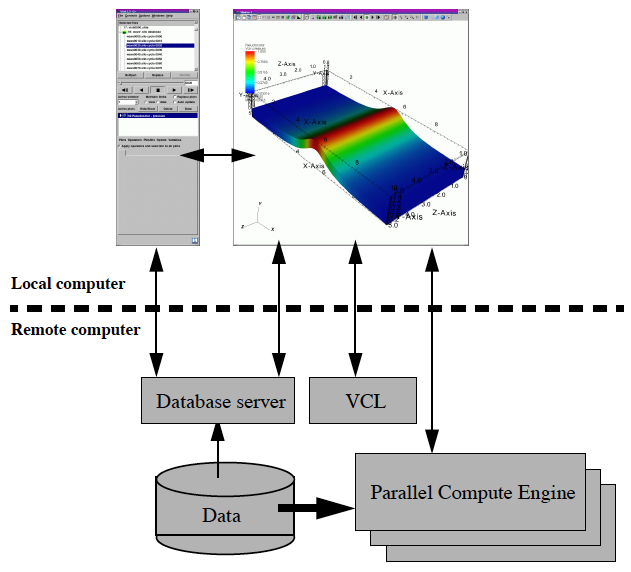
\includegraphics[width=\columnwidth]{figs/visit-guis/VisIt_arch}
    \end{column}
    \begin{column}{5.00cm}
      \begin{itemize}\setlength{\itemsep}{3mm}
      \item{\footnotesize Your local VisIt will start remote VCL (VisIt Component Launcher) responsible
        for launching other remote VisIt components}
      \item{\footnotesize Require:}
        \begin{enumerate}\setlength{\itemsep}{0mm}
        \item{\scriptsize properly configured VisIt on the HPC system}
        \item{\scriptsize a host profile (configured by HPC support staff) to tell your local VisIt
          how to connect and how to launch VCL on the HPC system (could be a queued job)}
        \end{enumerate}
      \end{itemize}
    \end{column}
  \end{columns}
\end{frame}

\defverbatim[colored]\batchOne{
  \begin{lstlisting}[language=bash,basicstyle=\scriptsize,keywordstyle=\color{red}]
qsub -q interactive -I -l nodes=1:ppn=1:gpus=1,walltime=1:00:00
... wait for an interactive shell ...
firstgpu=$( head -n 1 "$PBS_GPUFILE" )
gpuindex=${firstgpu:(-1)}
export DISPLAY=:0.$gpuindex
/global/software/visit/visit271/bin/visit -nowin -cli -s script.py
  \end{lstlisting}
}

\defverbatim[colored]\batchTwo{
  \begin{lstlisting}[language=bash,basicstyle=\scriptsize,keywordstyle=\color{red}]
qsub -q interactive ./visualization.sh
--- visualization.sh ---
#!/bin/bash
#PBS -S /bin/bash
#PBS -q gpu
#PBS -l nodes=1:ppn=4:gpus=1
#PBS -l pmem=2000mb
#PBS -l walltime=01:00:00
cd $PBS_O_WORKDIR
firstgpu=$( head -n 1 "$PBS_GPUFILE" )
gpuindex=${firstgpu:(-1)}
export DISPLAY=:0.$gpuindex
/global/software/visit/visit271/bin/visit -np 4 -nowin -cli -s script.py
  \end{lstlisting}
}

\begin{frame}{Batch scripting on HPC: examples on parallel.westgrid.ca}
  \underline{Example 1:} serial rendering via a scheduled interactive job
  \batchOne
  \underline{Example 2:} parallel rendering via a scheduled batch job
  \batchTwo
\end{frame}

%% parallel
%% qsub -q interactive -I -l nodes=1:ppn=4:gpus=1,walltime=0:30:00
%% visit -l mpirun -np 4     # will it print the port #?
%% need to recompile the MPI version?

%% laptop
%% Options \ra Host profiles and Configuratin Setup
%% select None (use VisIt's standard defaults)
%% Options \ra Host profiles
%% cn0553
